\documentclass[12pt]{article}
\usepackage[margin=1.0in]{geometry}
\usepackage[utf8]{inputenc}
\usepackage{graphicx, subcaption}
\usepackage{biblatex-chicago}
\bibliography{resources}
%\usepackage{cite}

\begin{document}
{\centering \Large Simulated depth of field

 \normalsize Ryan Ramsdell, Devesh Sullivan, and Amanda Sarsha \par\null}


The aim of our application is to simulate a shallow depth of field in post production. Camera systems embedded in many consumer electronics like cell phones are generally smaller than traditional options. This reduced size in optics and sensor size puts limitations of the effective depth of field achievable, in result many of these systems are designed with a wider depth of field. Depth of field is critical in the artistic value of an image as it can be used as a powerful compositional tool in highlighting the subject matter or conversely obscuring unwanted parts of the image scene.

In attacking this problem we will initially restrict ourselves to an image domain with human subjects.  The rationale being that selfies and portraits make for a large share of images taken today. With an increasingly connected society the issue of having a strong and reputable social media presence has become even more common. Our intention is to address the matter of resource access inequality (i.e., having a quality camera or ability to hire professional photographers) by implementing a solution that requires minimal hardware or effort in the image capture phase but still produces quality results comparable to professional images. Additionally, in implementing a software solution to this problem we eliminate the need for costly hardware systems. 

The methodology can be broken into two distinct steps: image depth map calculation and rendering the final image. 

Several solutions have been proposed in generating an image depth map. Depth from focus\autocite{Nayar1994} and depth from defocus\autocite{Favaro2003} both rely on the ability to alter the focus of the system, either through manipulation of relative distance between the lens and the image sensor or by adjustments to the aperture. They are further limited by requiring more than one image in order to calculate depth. Achieving good depth-resolution needs even more images, although Nayar and Nakawaga\autocite{Nayar1994} suggest the use of Gaussian interpolation algorithms are sufficient to artificially increase resolution. Another approach is calculating depth from a pair of stereo images by examining disparity in matched scene points\autocite{Longuet-Higgins1981}. Longuet-Higgins assumes a known bijective correspondence between scene points in his methodology. Luckily this has been addressed by a multitude of parties, Scharstein and Szeliski\autocite{Scharstein2002} explore several algorithms that produce \textit{dense} disparity maps, in that each pixel has a corresponding disparity estimate. At the time of publishing, they suggested the simple-shiftable-window algorithm presented by Hirshchmüller\autocite{Hirschmuller2002} was the most efficient algorithm. They maintain a taxonomy of currently best ranked algorithms online. Among the top ranked is a continuous 3D label stereo matching method using local expansion moves proposed by Taniai, Matsushita, Sato, and Naeumura\autocite{Taniai2016}. This proposed method relies on an iterative approach with graph cuts used to propagate small changes in a localized area (3x3 cell). It is very slick in its approach but relies on Markov random fields and is outside of our scope to be implemented in time. Other approaches include image segmentation and dual-pixel autofocus systems operating on single images, both explored by Wadhwa et al.\autocite{Wadhwa2018}. Image segmentation generally makes assumptions about the scene trying to be captured and can use neural networks or other methods to separate common subject matter like people. The dual-pixel autofocus relies on specific sensor hardware and is not adaptable to most situations. Another segmentation technique proposed by Battiato et al.\autocite{Battiato2004} performs color based image segmentation, then labels areas based on predetermined classifications gathered by examining common indoor and outdoor scenes and finally combines this with geometric properties to estimate the depth map.

Blurring and image composition present additional design decisions. As an aside, Wadhwa et al\autocite{Wadhwa2018} give a naïve but accurate approach where each scene point projects a translucent disk (a scatter convolution of sorts) in the image with depths stacked as appropriate. This method is eschewed by the authors because it is computationally expensive on mobile phones and other low powered devices. Instead they offer a gather convolution coupled with a faster scatter convolution over a circle rather than a disk (filled circle) and a few other optimizations to make it run as quickly as possibly while still producing acceptable results. Other research has been done to create a circular separable convolution such using Gaussians like those produced by Garcia\autocite{Garcia2017} or Niemitalo\autocite{Niemitalo2010}. These approximate a perfectly circular blur disk produced by a perfectly circular aperture in a real lens and are very fast to compute. The näive approach suggested by Wadhwa\autocite{Wadhwa2018} is more extensible in that it is easier to produce non-circular blur disks such as the hexagonal ones produced by physical camera systems with six-blade apertures.

Wholesale solutions to the problem also exist and are actively being researched by major phone and camera software producers. In particular, the portrait mode implemented by Google in their camera app for Android phones utilizes artificial intelligence to generate depth maps and create false depth of field\autocite{Hernandez2014}. They use a Structure From Motion technique with Markov random field inference methods to calculate the depth map and rendering was done by using the thin lens approximation. Apple has a similar product.

Our approach will use the segmentation technique given by Wadhwa et al.\autocite{Wadhwa2018} as it is most adaptable to any imaging system which aligns with our general goal of being a hardware independent system. We are researching the ability to use Haar feature search and either mean-shift or graph based image segmentation to separate a human subject from the background of an image. The Haar algorithm would find the human subject and we intend to adjust the segmentation parameters so that the face we've recognized stays in one segment. After segmentation we will rely on reasonable assumptions about image composition that should more in most cases. Namely that the human subject will be in the foreground and that all other parts will be behind the subject. In addition, the if we have segments that are at different vertical heights along the image, the ones closer to the top will be assumed to be further from the camera as is true with a distant horizon or sky. Segmentation is limited in how many objects it can discern so we will also use Gaussian interpolation as suggested by Nayar et al. \autocite{Nayar1994} as a way of increasing the depth-resolution. If time permits we may explore additional depth-map calculation techniques like depth from focus/defocus with images gathered from short video segments with changing focus or implementing an algorithm to gather depth from stereo.

We also plan to implement the more photorealistic image rendering technique from Wadhwa et al. \autocite{Wadhwa2018}  over the faster Gaussian approximations suggested by Garcia\autocite{Garcia2017} and Niemitalo.\autocite{Niemitalo2010} The current algorithm masks the image for each depth value and blurs with a circle of confusion proportional to the distance from the focal plane. We have restricted it to an only 8-bit depth-map which is expected to be fine given the limited resolution in our depth-map calculations. This keeps our render time down significantly. Focus is chosen manually at the moment, although it should be easy to automatically focus on the assumed human subject when our depth map calculations have been fully implemented as it designed to specifically look for human faces. We have the additional hope of allowing for arbitrary aperture shape, which requires updating our blur kernel generation algorithm to produce other shapes. In this consideration we will need to decide between procedurally generated shapes or up/down scaling pre-made kernel assets. Preliminary results can be seen in figure \ref{fig:blur1}.

Currently we are using computer generated images to run tests in a controlled setting. With this we have the advantage of producing images of scenes with perfectly accurate and precise depth map calculations for which we can compare our own depth map against, as well as fine tuning the image composition section using said map. A future framework we wish to test our depth map algorithm are the datasets available from the taxonomy maintained on the Middlebury College website.\autocite{Scharstein2002}\autocite{Scharstein2003}\autocite{Scharstein2007}\autocite{Scharstein2014}\autocite{Hirschmuller2007} These tests will provide us with quantatative data to evaluate the effectiveness of our images. Furthermore we will test the accuracy of our segmentation and rendering phases on real-life stills by taking multiple stills of a scene with varying depth of field on a digital single lens reflex camera and comparing the results of our solution applied to the wide depth of field shots with the shallower optical results. 

Moving forward, we still have to implement the depth-map calculation. Ideally this will be done by mid-November so that we can thoroughly test our application and then begin working on supplementary parts and fine-tuning the overall product. 

\pagebreak
\begin{figure}[h!]
  \centering
  \begin{subfigure}[b]{0.4\linewidth}
    \includegraphics[width=\linewidth]{img_rend.png}
    \caption{Original image.}
  \end{subfigure}
  \begin{subfigure}[b]{0.4\linewidth}
    \includegraphics[width=\linewidth]{img_depth.png}
    \caption{Image depth map.}
  \end{subfigure}
  \begin{subfigure}[b]{0.55\linewidth}
    \includegraphics[width=\linewidth]{render.png}
    \caption{Final composited imaged.}
  \end{subfigure}
  
  \begin{subfigure}[b]{0.4\linewidth}
    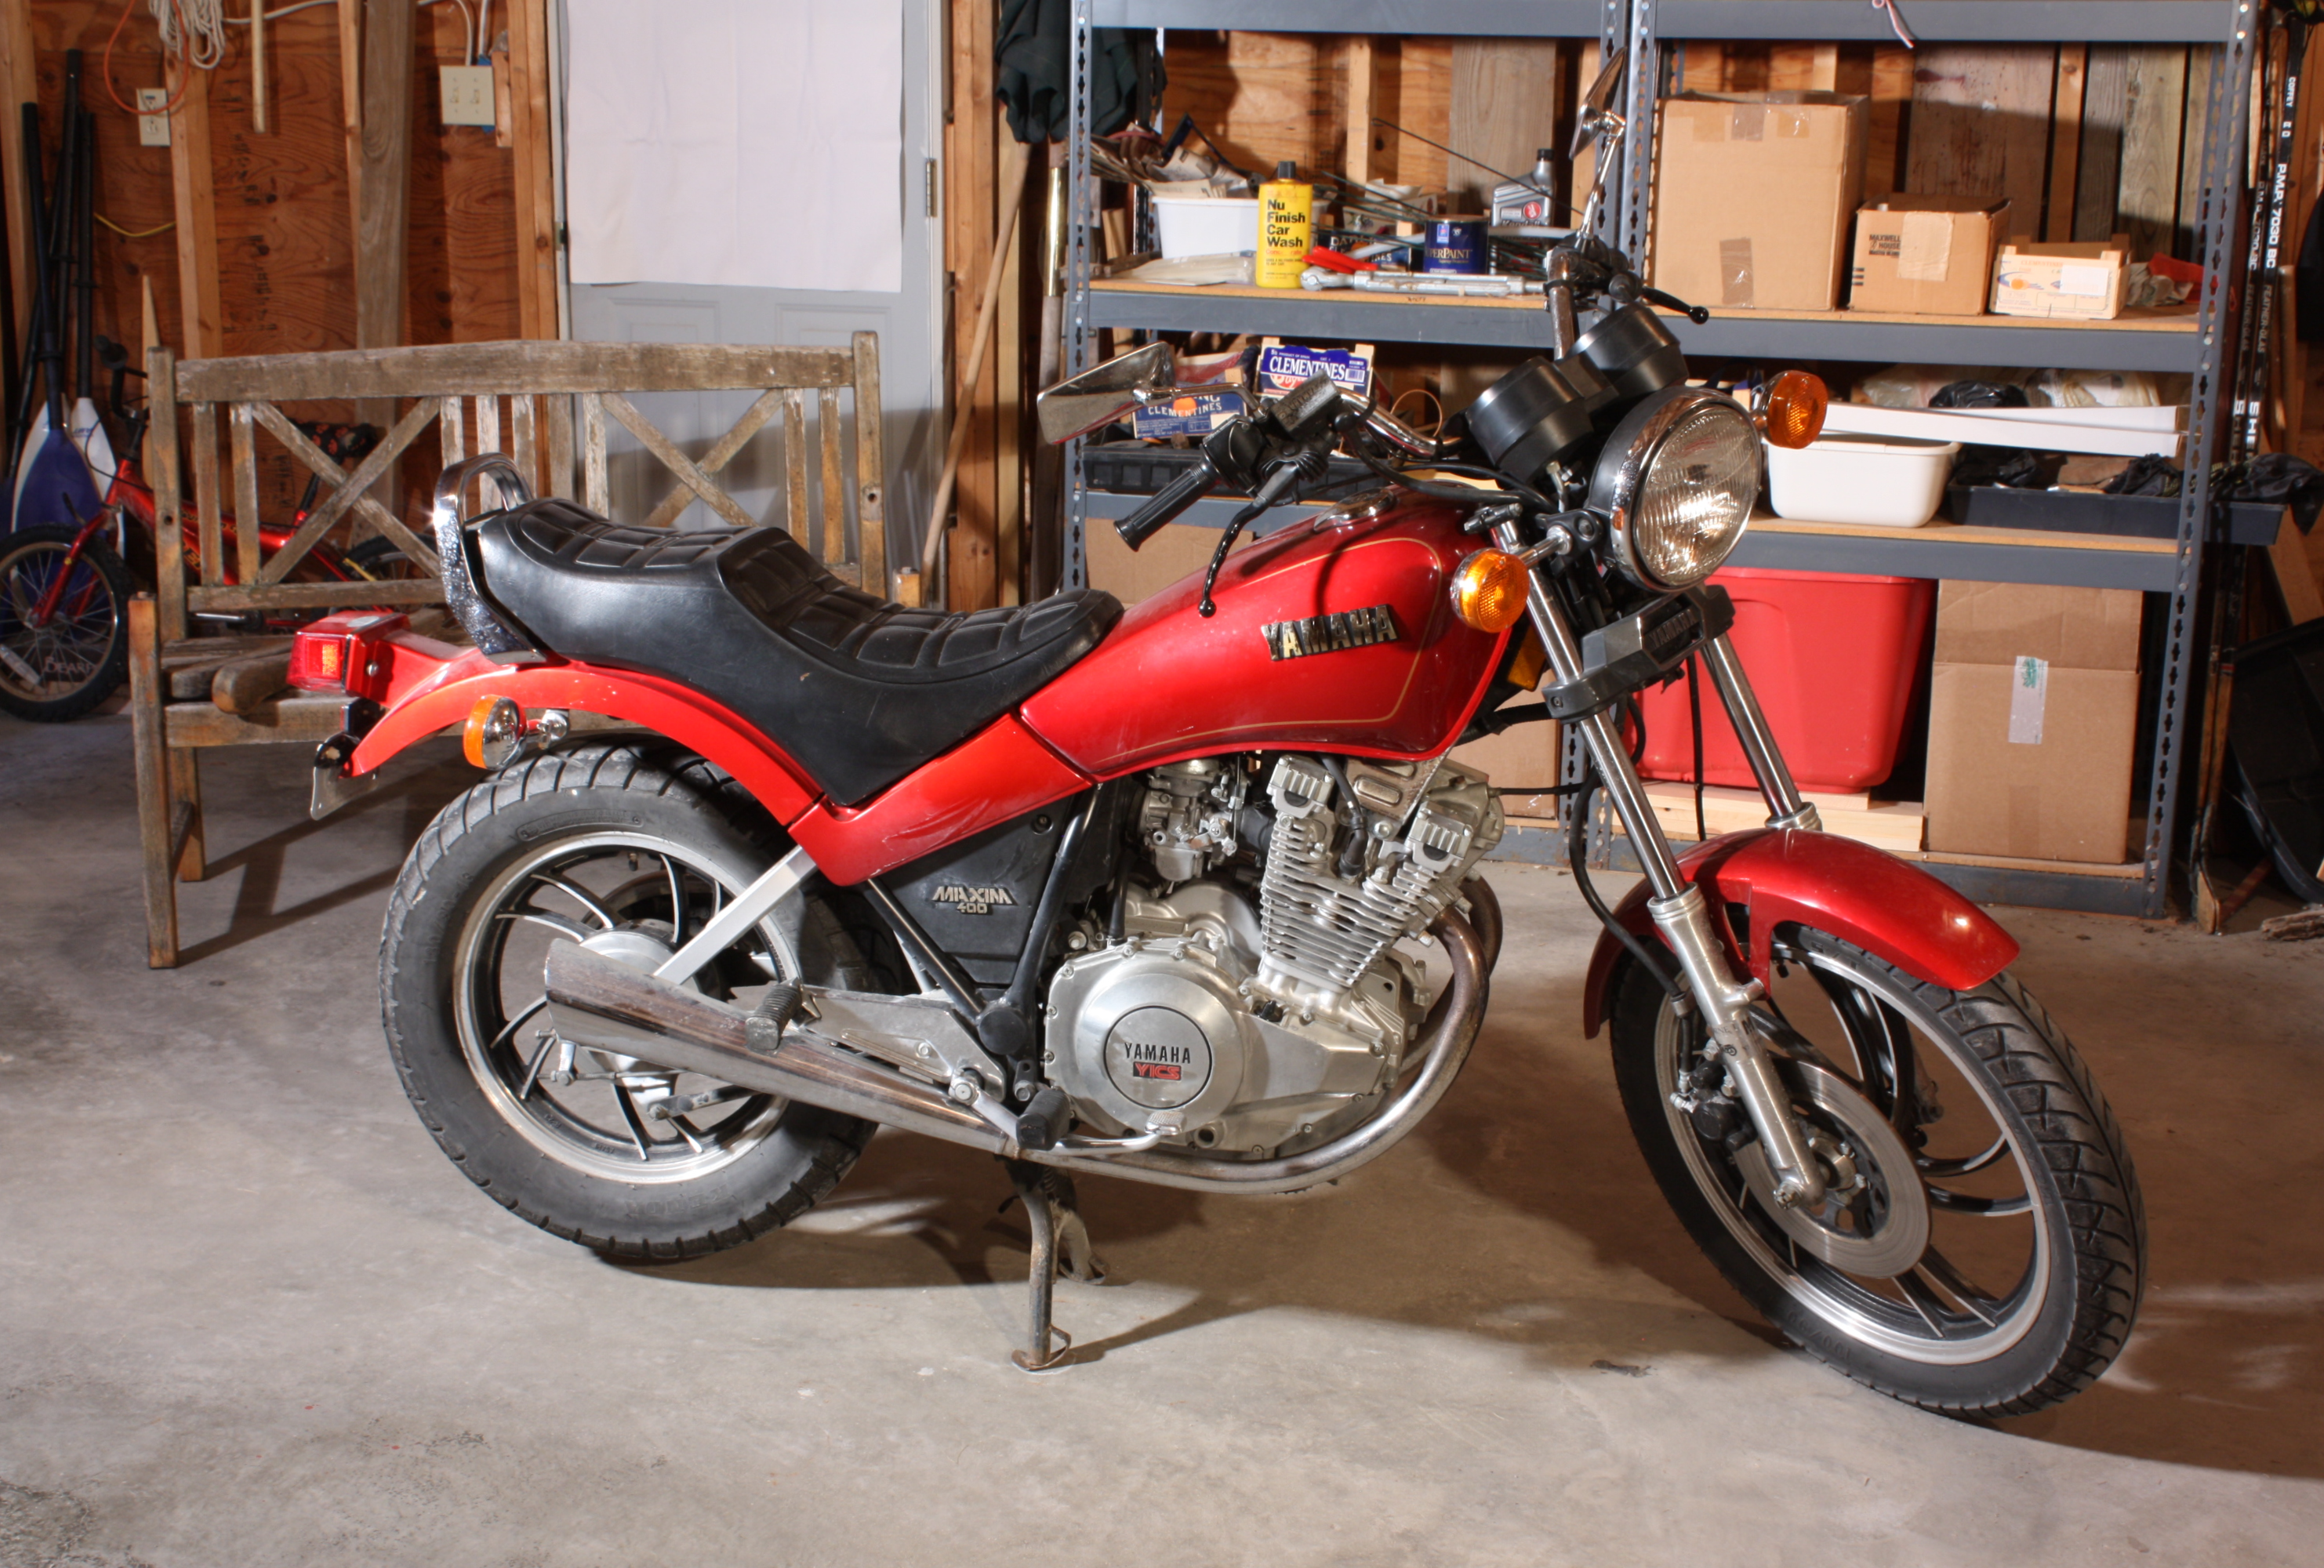
\includegraphics[width=\linewidth]{moto.png}
    \caption{Original image.}
  \end{subfigure}
  \begin{subfigure}[b]{0.4\linewidth}
    \includegraphics[width=\linewidth]{moto_d.png}
    \caption{Image depth map.}
  \end{subfigure}
  \begin{subfigure}[b]{0.55\linewidth}
    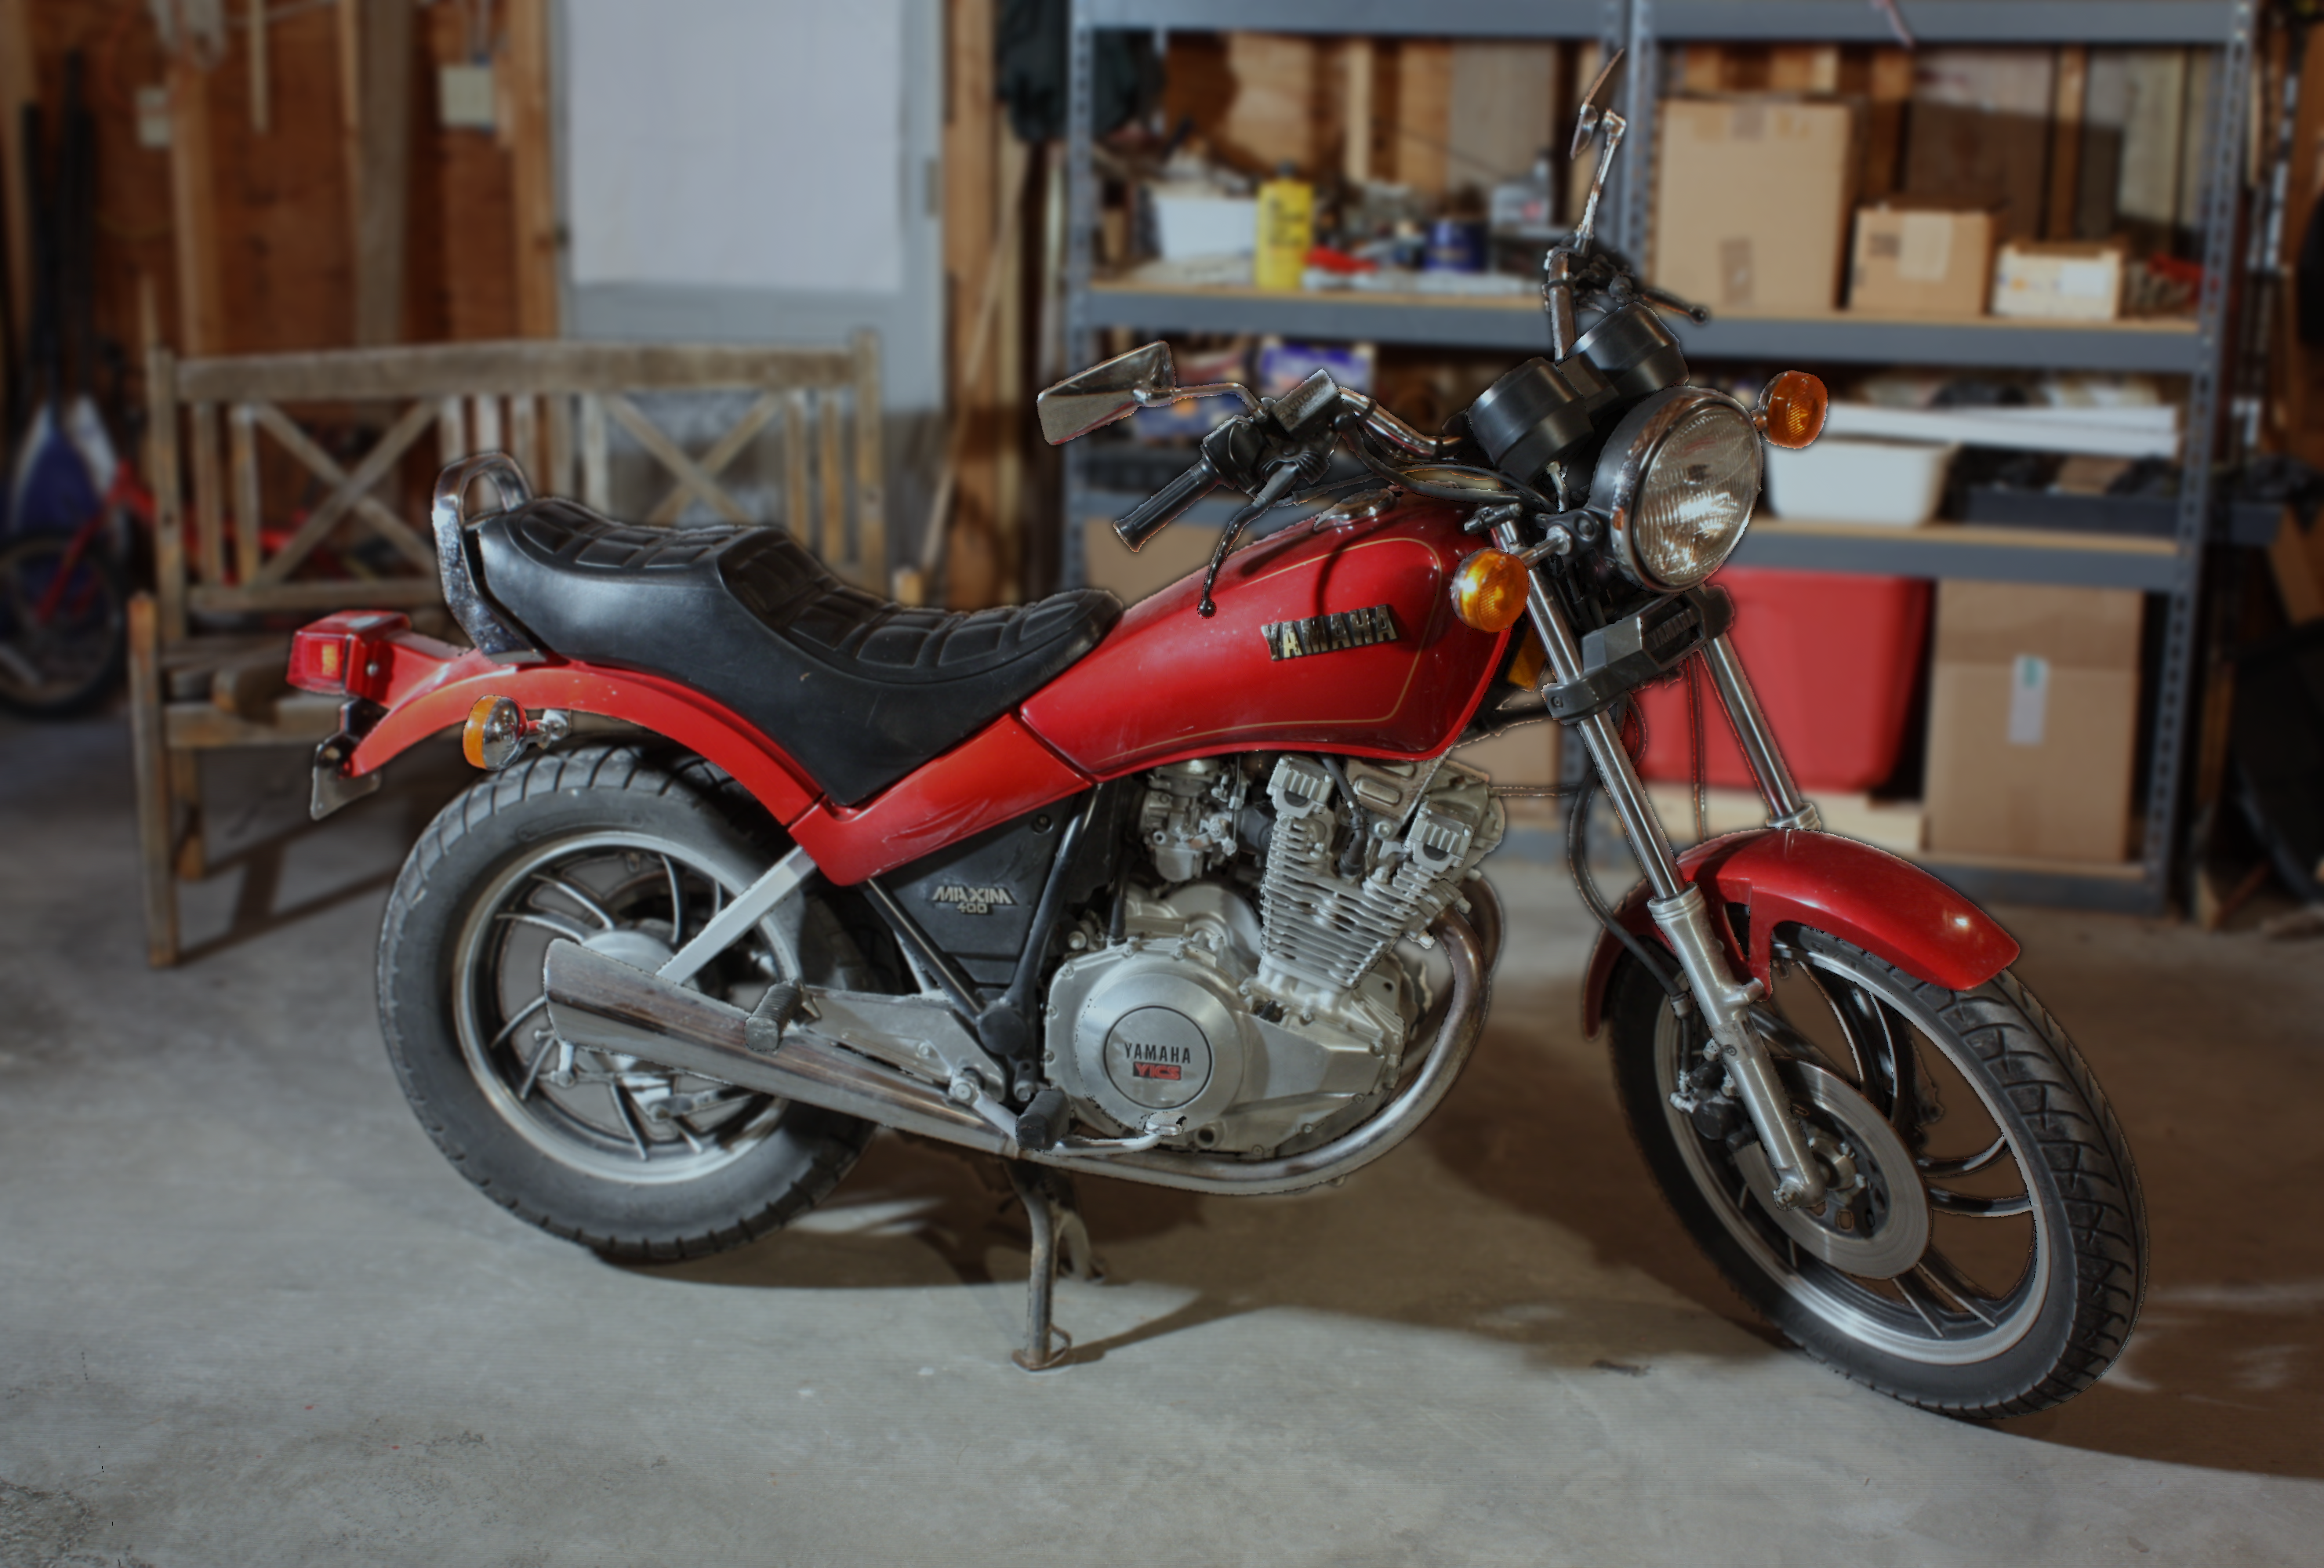
\includegraphics[width=\linewidth]{render2.png}
    \caption{Final composited imaged.}
  \end{subfigure}

  \caption{Simulated depth of focus by blurring pixels based on depth.}
  \label{fig:blur1}
\end{figure}




\clearpage
\printbibliography[heading=bibintoc]

\end{document}